%!TEX root = guide2.0.tex


\section*{An example statistical model}
Consider the following dataset, which is a time series of recorded coal mining disasters in the UK from 1851 to 1962 (\cite{Jarrett:1979fr}).
\begin{center}
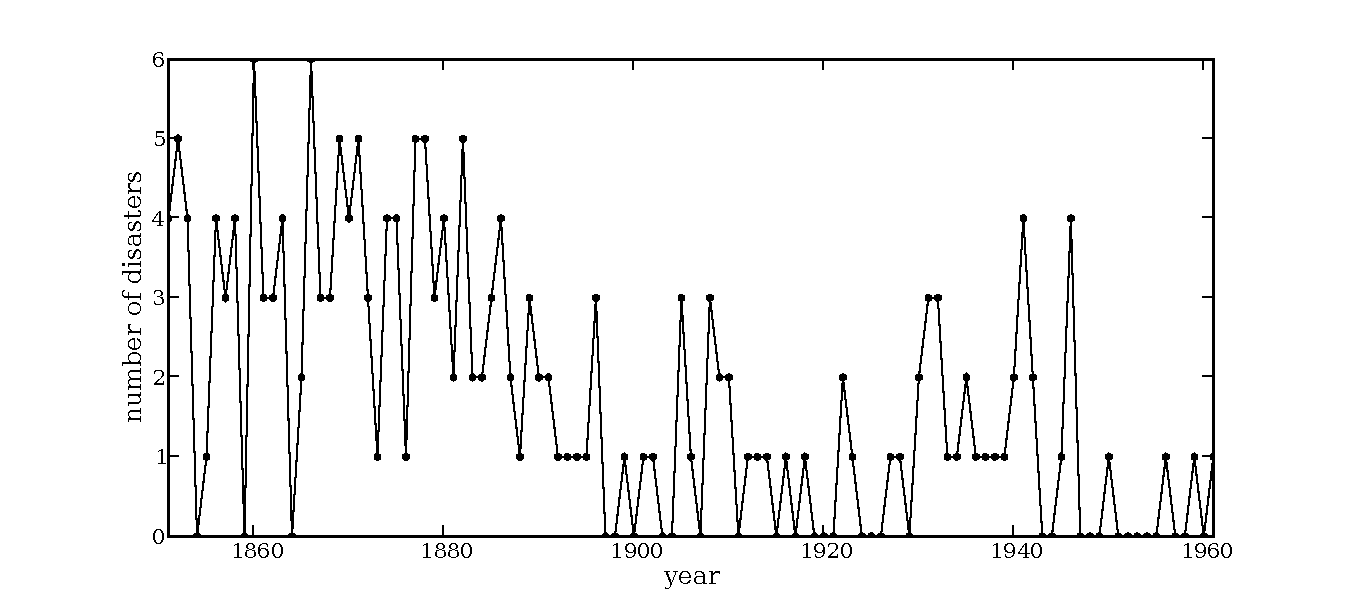
\epsfig{file=disasterts.pdf, width=15cm}
\end{center}
Occurrences of disasters in the time series is thought to be derived from a Poisson process with a large rate parameter in the early part of the time series, and from one with a smaller rate in the later part. We are interested in locating the change point in the series, which perhaps is related to changes in mining safety regulations.

We represent our conceptual model formally as a statistical model:
\begin{equation}
    \begin{array}{ccc}
        (D_t | s, e, l) \sim \textup{Poisson}\left(r_t\right), & r_t=\left\{\begin{array}{lll}
            e &\texttt{for}& t< s\\ l &\texttt{ for}& t\ge s
            \end{array}\right.,&t\in[t_l,t_h]\\
        s\sim \textup{Uniform}(t_l, t_h)\\
        e\sim \textup{Exponential}(r_e)\\
        l\sim \textup{Exponential}(r_l)        
    \end{array}
    \label{disastermodel} 
\end{equation}
The symbols have the following meanings:
\begin{description}
    \item[$D_t$:] The number of disasters in year $t$.
    \item[$r_t$:] The rate parameter of the Poisson distribution of disasters in year $t$.
    \item[$s$:] The year in which the rate parameter changes (the switchpoint).
    \item[$e$:] The rate parameter before the switchpoint $s$.
    \item[$l$:] The rate parameter after the switchpoint $s$.
    \item[$t_l$ and $t_h$:] The lower and upper boundaries of year $t$.
    \item[$\beta_e$ and $\beta_l$:] Prior parameters (also called hyperparameters).
\end{description}
Because we have defined $D$ by its dependence on $s$, $e$ and $l$, the latter three are known as the `parents' of $D$ and $D$ is called their `child'. Similarly, the parents of $s$ are $t_l$ and $t_h$, and $s$ is the child of $t_l$ and $t_h$.

\section*{Conditionally stochastic and conditionally deterministic variables}

At the model-specification stage (before the data have been observed), $D$, $s$, $e$, $r$ and $l$ are all \emph{random} variables. Under the Bayesian interpretation of probability, \emph{random} variables have not necessarily arisen from a physical random process. Instead, probability distributions are used to characterize our uncertainty in the true parameter values. Random variables are represented in PyMC by \code{Stochastic} and \code{Deterministic} classes (Both \code{Stochastic} and \code{Deterministic} are subclasses of the generic \code{Variable} class). There is a difference between $r$ and the other variables: if we knew the values of $r$'s parents, we could compute the value of $r$ exactly. This variable, represented by the \code{Deterministic} class, is defined by a mathematical function which returns its value given values for its parents. This nomenclature is a bit confusing, because these objects usually represent random variables; if the parents of $r$ are random, $r$ is random also. A more descriptive (though more awkward) name for this class would be \code{DeterminedByValuesOfParents}.

On the other hand, even if the values of the parents of parameters $s$, $D$, $e$ or $l$ were known, we would still be uncertain of their values. These variables are characterized by probability distributions that express how plausible their candidate values are, given values for their parents. The \code{Stochastic} class represents these variables. A better name for these objects might be \code{RandomEvenGivenValuesOfParents}.

We can represent model \ref{disastermodel} in a file called \module{DisasterModel.py} as follows. First, we import the PyMC and NumPy namespaces and enter the actual data values into an array:
\begin{verbatim}
	
from pymc import DiscreteUniform, Exponential, deterministic, Poisson, Uniform
import numpy as np

disasters_array =   np.array([ 4, 5, 4, 0, 1, 4, 3, 4, 0, 6, 3, 3, 4, 0, 2, 6,
                   3, 3, 5, 4, 5, 3, 1, 4, 4, 1, 5, 5, 3, 4, 2, 5,
                   2, 2, 3, 4, 2, 1, 3, 2, 2, 1, 1, 1, 1, 3, 0, 0,
                   1, 0, 1, 1, 0, 0, 3, 1, 0, 3, 2, 2, 0, 1, 1, 1,
                   0, 1, 0, 1, 0, 0, 0, 2, 1, 0, 0, 0, 1, 1, 0, 2,
                   3, 3, 1, 1, 2, 1, 1, 1, 1, 2, 4, 2, 0, 0, 1, 4,
                   0, 0, 0, 1, 0, 0, 0, 0, 0, 1, 0, 0, 1, 0, 1])
\end{verbatim} 
Next, we create the switchpoint variable $s$:
\begin{verbatim}
	s = DiscreteUniform('s', lower=0, upper=110, doc='Switchpoint
[year]')  
\end{verbatim}
\code{DiscreteUniform} is a subclass of \code{Stochastic} that represents uniformly-distributed discrete variables. Use of this distribution suggests that we have no information \emph{a priori} regarding the location of the switchpoint; all values are equally likely. Now we create the exponentially-distributed variables $e$ and $l$:
\begin{verbatim}
   	e = Exponential('e', beta=1)
	l = Exponential('l', beta=1)   
\end{verbatim}
Next, we define the variable $r$, which selects the early rate $e$ for times before $s$ and the late rate $l$ for times after $s$. We create $r$ using the \code{deterministic} decorator, which converts the ordinary Python function $r$ into a \code{Deterministic} object.
\begin{verbatim}
	@deterministic(plot=False)
	def r(s=s, e=e, l=l):
		""" Concatenate Poisson means """
	    out = np.empty(len(disasters_array))
	    out[:s] = e
	    out[s:] = l
	    return out
\end{verbatim}
The last step is to define the number of disasters $D$. This is done the same way as for stochastic variables, except that we set the argument \code{isdata} to \code{True} (it is set to \code{False} by default). This tells PyMC that this object has a fixed value and does not need to be sampled:
\begin{verbatim}
	D = Poisson('D', mu=r, value=disasters_array, isdata=True)
\end{verbatim}

\subsection*{Why are data and unknown variables represented by the same object?}
Since it is represented by a \code{Stochastic} object, $D$ is defined by its dependence on its parents $s$, $e$ and $l$ even though its value is fixed. This isn't just a quirk of PyMC's syntax; Bayesian hierarchical notation itself makes no distinction between random variables and data. The reason is simple: to use Bayes' theorem to compute the posterior $p(e,s,l|D)$ of model \ref{disastermodel}, we need to use the likelihood $p(D|e,s,l)$. Even though $D$'s value is known and fixed, we need to formally assign it a probability distribution as if it were a random variable.

This point can be counterintuitive at first, as many peoples' instinct is to regard data as fixed a priori and unknown variables as dependent on the data. One way to understand this is to think of statistical models like (\ref{disastermodel}) as predictive models for data, or as models of the processes that gave rise to data. Before observing the value of $D$, we could have sampled from its prior predictive distribution $p(D)$ (\emph{i.e.} the marginal distribution of the data) as follows:
\begin{enumerate}
    \item Sample $e$, $s$ and $l$ from their priors.
    \item Sample $D$ conditional on these values.
\end{enumerate}
Even after we observe the value of $D$, we need to use this process model to make inferences about $e$, $s$ and $l$; it's the only information we have about how the variables are related.

\medskip
To look at the issue another way, we could, in principle, have written a model equivalent to (\ref{disastermodel}) such that $D$ depended on nothing and everything else depended on $D$, for example
\begin{eqnarray*}
    s|e,l,D\sim\cdot\\
    e|l,D\sim\cdot\\
    l|D\sim\cdot\\
    D=D_*
\end{eqnarray*}

In one respect, this would have been more natural because we would have the unknown stochastic variables depending on the data. However, if we could write down that model using standard distributions we could trivially compute and sample from the posterior,
\begin{eqnarray*}
    p(s,e,l|D) = p(s|e, l, D) p(e|l, D) p(l|D),
\end{eqnarray*}
and we would have no use for MCMC or any other fitting method. Bayesian methods, and statistics in general, are needed when it's feasible to write down the data's dependence on the unknown variables but not vice versa.


\section*{Parents and children}

We have created a PyMC probability model, which is simply a linked collection of variables. To see the nature of the links, import or run \code{DisasterModel.py} and examine $s$'s \code{parents} attribute from the Python prompt:
\begin{verbatim}
   >>> s.parents
   >>> {'lower': 0, 'upper': 110}
\end{verbatim}
The \code{parents} dictionary shows us the distributional parameters of $s$. Now try examining $D$'s parents:
\begin{verbatim}
   >>> D.parents
   >>> {'mu': <pymc.PyMCObjects.Deterministic 'r' at 0x3e51a70>}
\end{verbatim}
We are using $r$ as a distributional parameter of $D$, so $r$ is $D$'s parent. $D$ labels $r$ as \code{mu}, meaning it plays the role of the rate parameter in $D$'s Poisson distribution. Now examine $r$'s \code{children} attribute:
\begin{verbatim}
   >>> r.children
   >>> set([<pymc.distributions.Poisson 'D' at 0x3e51290>])
\end{verbatim}
Because $D$ considers $r$ its parent, $r$ considers $D$ its child. Unlike \code{parents}, \code{children} is a set; variables do not associate their children with any particular distributional role. Try examining the \code{parents} and \code{children} attributes of the other parameters in the model.

\begin{center}
   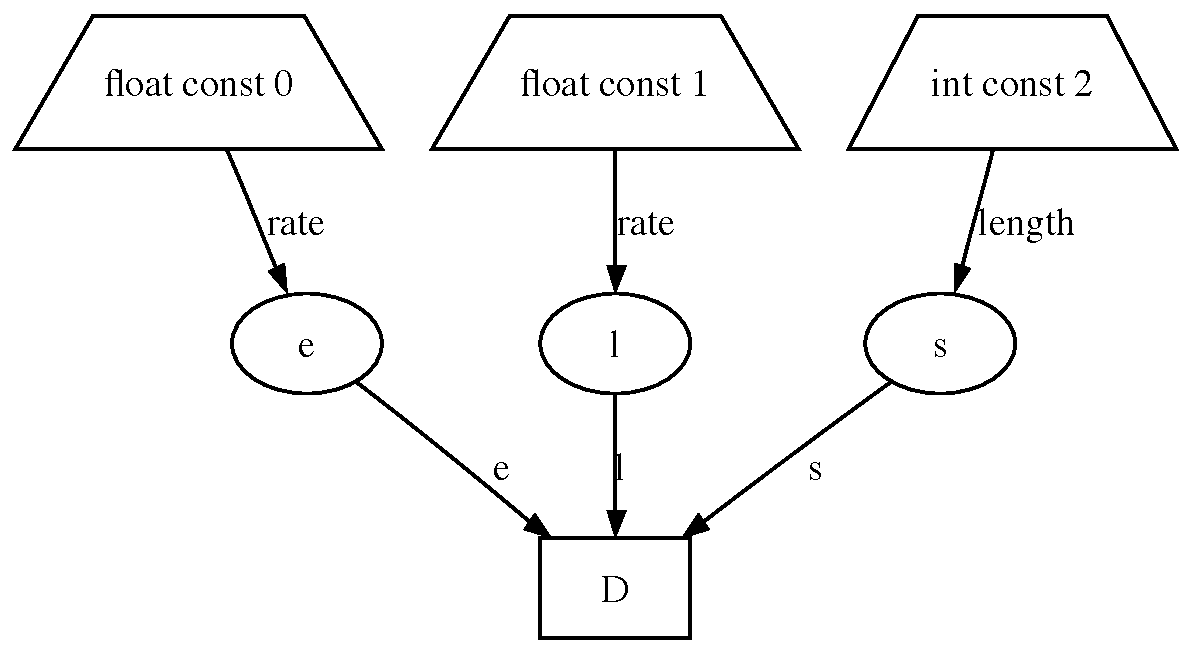
\epsfig{file=DisasterModel.pdf, width=5cm}
\end{center}

\section*{Variables' values and log-probabilities}
All PyMC variables have an attribute called \code{value}. Try examining $D$'s value, and you'll see the initial value we provided for it:
\begin{verbatim}
   >>> D.value
   >>> 
   array([4, 5, 4, 0, 1, 4, 3, 4, 0, 6, 3, 3, 4, 0, 2, 6, 3, 3, 5, 4, 5, 3, 1,
          4, 4, 1, 5, 5, 3, 4, 2, 5, 2, 2, 3, 4, 2, 1, 3, 2, 2, 1, 1, 1, 1, 3,
          0, 0, 1, 0, 1, 1, 0, 0, 3, 1, 0, 3, 2, 2, 0, 1, 1, 1, 0, 1, 0, 1, 0,
          0, 0, 2, 1, 0, 0, 0, 1, 1, 0, 2, 3, 3, 1, 1, 2, 1, 1, 1, 1, 2, 4, 2,
          0, 0, 1, 4, 0, 0, 0, 1, 0, 0, 0, 0, 0, 1, 0, 0, 1, 0, 1])
\end{verbatim}
If you check $e$'s, $s$'s and $l$'s values, you'll see random initial values generated by PyMC:
\begin{verbatim}
   >>> s.value
   >>> 44

   >>> e.value
   >>> 0.33464706250079584

   >>> l.value
   >>> 2.6491936762267811
\end{verbatim}
Of course, since these are \code{Stochastic} elements, your value will be different than these. If you check $r$'s value, you'll see an array whose first $s$ elements are \code{e.value}, and whose remaining elements are \code{l.value}:
\begin{verbatim}
   >>> r.value
   >>> 
   array([ 0.33464706,  0.33464706,  0.33464706,  0.33464706,  0.33464706,
           0.33464706,  0.33464706,  0.33464706,  0.33464706,  0.33464706,
           0.33464706,  0.33464706,  0.33464706,  0.33464706,  0.33464706,
           0.33464706,  0.33464706,  0.33464706,  0.33464706,  0.33464706,
           0.33464706,  0.33464706,  0.33464706,  0.33464706,  0.33464706,
           0.33464706,  0.33464706,  0.33464706,  0.33464706,  0.33464706,
           0.33464706,  0.33464706,  0.33464706,  0.33464706,  0.33464706,
           0.33464706,  0.33464706,  0.33464706,  0.33464706,  0.33464706,
           0.33464706,  0.33464706,  0.33464706,  0.33464706,  2.64919368,
           2.64919368,  2.64919368,  2.64919368,  2.64919368,  2.64919368,
           2.64919368,  2.64919368,  2.64919368,  2.64919368,  2.64919368,
           2.64919368,  2.64919368,  2.64919368,  2.64919368,  2.64919368,
           2.64919368,  2.64919368,  2.64919368,  2.64919368,  2.64919368,
           2.64919368,  2.64919368,  2.64919368,  2.64919368,  2.64919368,
           2.64919368,  2.64919368,  2.64919368,  2.64919368,  2.64919368,
           2.64919368,  2.64919368,  2.64919368,  2.64919368,  2.64919368,
           2.64919368,  2.64919368,  2.64919368,  2.64919368,  2.64919368,
           2.64919368,  2.64919368,  2.64919368,  2.64919368,  2.64919368,
           2.64919368,  2.64919368,  2.64919368,  2.64919368,  2.64919368,
           2.64919368,  2.64919368,  2.64919368,  2.64919368,  2.64919368,
           2.64919368,  2.64919368,  2.64919368,  2.64919368,  2.64919368,
           2.64919368,  2.64919368,  2.64919368,  2.64919368,  2.64919368])
\end{verbatim}
To compute its value, $r$ calls the funtion we used to create it, passing in the values of its parents.

\code{Stochastic} objects can evaluate their probability mass or density functions at their current values given the values of their parents. The logarithm of a stochastic object's probability mass or density can be accessed via the \code{logp} attribute. For vector-valued variables like $D$, the \code{logp} attribute returns the log of the joint probability or density of all elements of the value. Try examining $s$'s and $D$'s log-probabilities and $e$'s and $l$'s log-densities:
\begin{verbatim}
   >>> s.logp
   >>> -4.7095302013123339

   >>> D.logp
   >>> -1080.5149888046033

   >>> e.logp
   >>> -0.33464706250079584

   >>> l.logp
   >>> -2.6491936762267811
\end{verbatim}
\code{Stochastic} objects need to call an internal function to compute their \code{logp} attributes, as $r$ needed to call an internal function to compute its value. Just as we created $r$ by decorating a function that computes its value, it's possible to create custom \code{Stochastic} objects by decorating functions that compute their log-probabilities or densities (see chapter \ref{chap:modelbuilding}). Users are thus not limited to the set of of statistical distributions provided by PyMC.

\subsection*{Using \code{Variables} as parents of \code{Variables}}

Let's take a closer look at our definition of $r$:
\begin{verbatim}
   	@deterministic(plot=False)
	def r(s=s, e=e, l=l):
	    """ Concatenate Poisson means """
	    out = np.empty(len(disasters_array))
	    out[:s] = e
	    out[s:] = l
	    return out
\end{verbatim}
The arguments are \code{Stochastic} objects, not numbers. Why aren't errors raised when we attempt to slice array \code{out} up to a \code{Stochastic} object?

Whenever a variable is used as a parent for a child variable, PyMC replaces it with its \code{value} attribute when the child's value or log-probability is computed. When $r$'s value is recomputed, \code{s.value} is passed to the function as argument \code{s}. To see the values of the parents of $r$ all together, look at \code{r.parents.value}.

\section*{Fitting the model with MCMC}

PyMC provides several objects that fit probability models (linked collections of variables) like ours. The primary such object, \code{MCMC}, fits models with the Markov chain Monte Carlo algorithm. See chapter \ref{chap:MCMC} for an introduction to the algorithm itself. To create an \code{MCMC} object to handle our model, import \module{DisasterModel.py} and use it as an argument for \code{MCMC}:
\begin{verbatim}
   import DisasterModel
   from pymc import MCMC
   M = MCMC(DisasterModel)
\end{verbatim}
To run the sampler, call the MCMC object's \code{isample()} (or \code{sample()}) method, either from \module{DisasterModel.py} or the prompt:
\begin{verbatim}
   M.isample(iter=10000, burn=1000)
\end{verbatim}
After a few seconds, you should see that sampling has finished normally. The model has been fitted.

\subsection*{What does it mean to fit a model?}

The MCMC sampler runs for the specified number of iterations. If the run is sufficiently long, the model will have converged to the posterior distribution of interest, and all subsequent samples can be considered samples from that distribution, and used for inference. The specified \code{burn} interval should be large enough to ensure that no pre-convergent samples are included in the sample used for generating summary statistics.

The output of the MCMC algorithm is a `trace', the sequence of retained samples for each variable in the model. These traces are stored as attributes of the variables themselves and can be accessed using the \code{trace()} method. For example:
\begin{verbatim}
   >>> s.trace()
   >>> array([41, 40, 40, ..., 43, 44, 44])
\end{verbatim}
The unknown variables $s$, $e$, $l$ and $r$ will all accrue samples, but $D$ will not because its value has been observed and is not updated.

\subsection*{Sampling output} 
You can examine the marginal posterior of any variable by plotting a histogram of its trace:
\begin{verbatim}
   >>> from pylab import hist, show
   >>> hist(l.trace())
   >>> 
   (array([   8,   52,  565, 1624, 2563, 2105, 1292,  488,  258,   45]),
    array([ 0.52721865,  0.60788251,  0.68854637,  0.76921023,  0.84987409,
           0.93053795,  1.01120181,  1.09186567,  1.17252953,  1.25319339]),
    <a list of 10 Patch objects>)
   >>> show()
\end{verbatim}
You should see something like this:
\begin{center}
   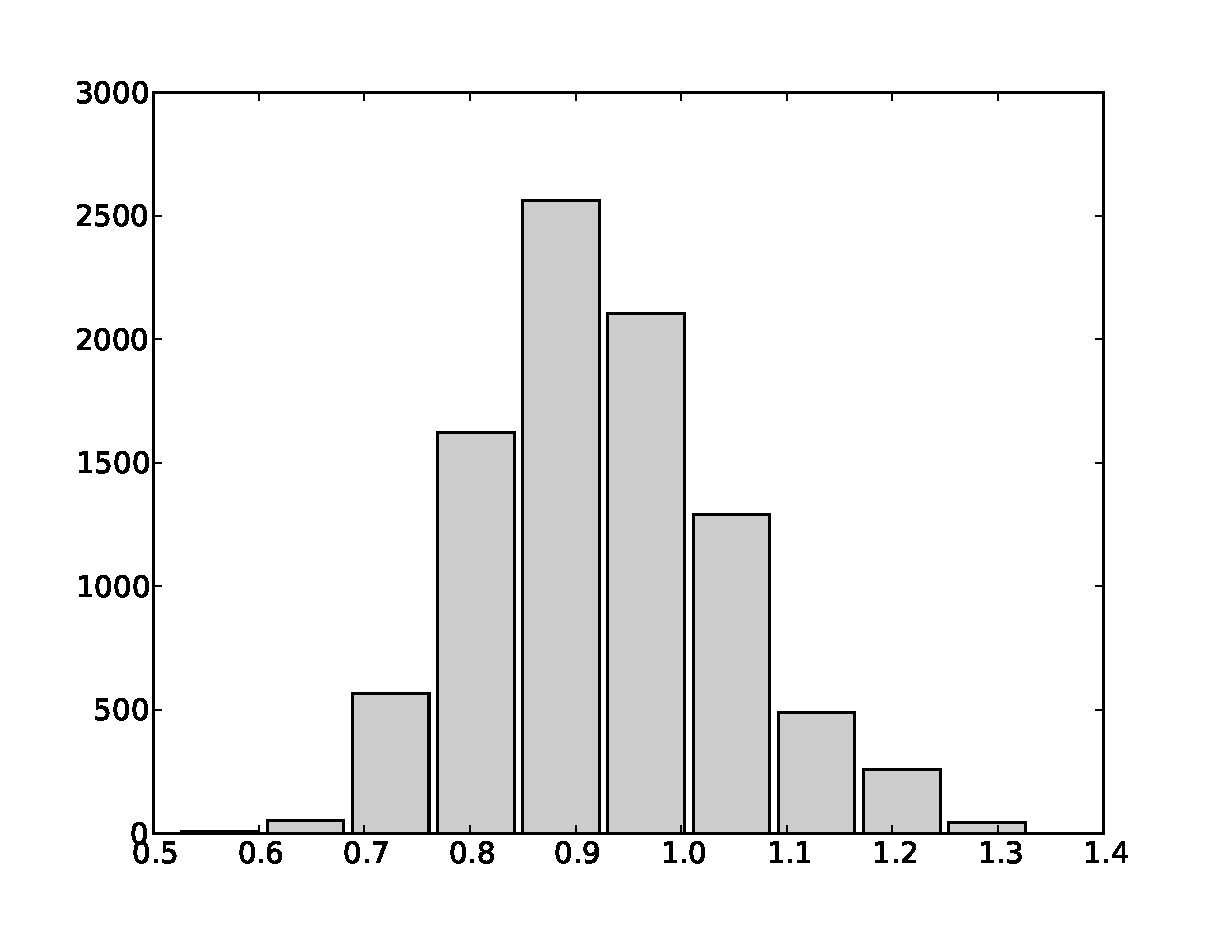
\epsfig{file=ltrace.pdf, width=10cm}
\end{center}
PyMC has its own plotting functionality, via the optional matplotlib module as noted in the installation notes. The \code{Matplot} module includes a \code{plot} function that takes the model (or a single parameter) as an argument:
\begin{verbatim}
   >>> from pymc.Matplot import plot
   >>> plot(M)
\end{verbatim}
You will see several figures like the following:
\begin{center}
   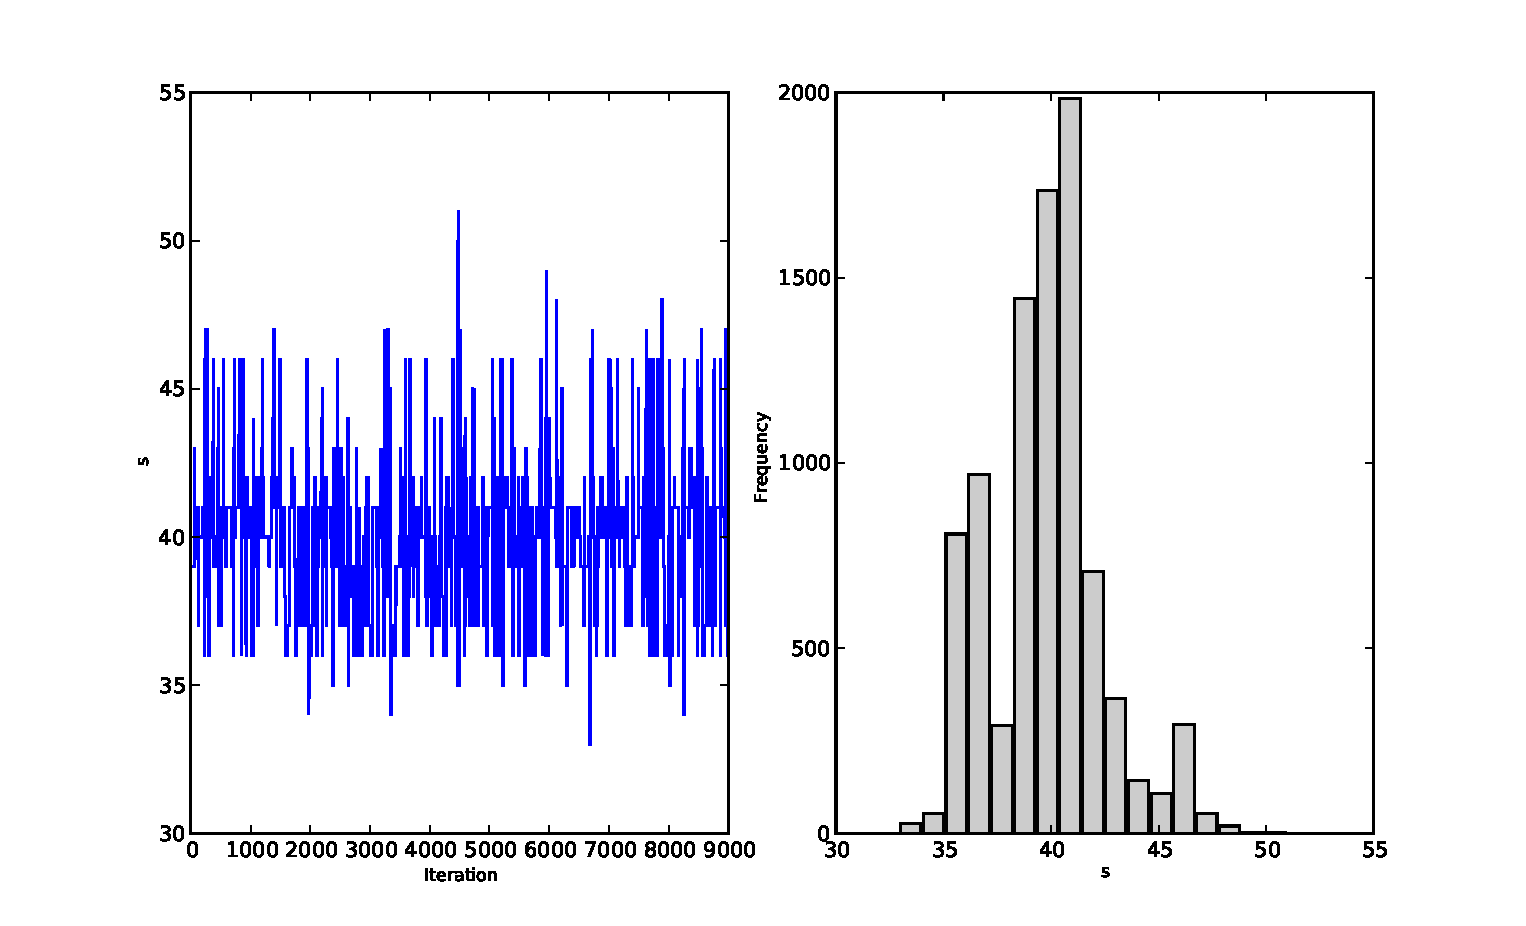
\epsfig{file=spost.pdf, width=15cm}
\end{center}
The left-hand pane of this figure shows the temporal series of the samples from $s$, while the right-hand pane shows a histogram of the trace. The trace is useful for evaluating and diagnosing the algorithm's performance [\textbf{ref}]. If the trace looks good, the right-hand pane is useful for visualizing the posterior. Notice that the posterior of $s$ appears to be bimodal.

For a non-graphical summary of the posterior, simply call \code{M.stats()}.


\section*{Fine-tuning the MCMC algorithm} 

MCMC objects handle individual variables via `step methods', which determine how parameters are updated at each step of the MCMC algorithm. By default, step methods are automatically assigned to variables by PyMC. To see which step methods $M$ is using, look at its \code{step_method_dict} attribute with respect to each parameter:
\begin{verbatim}
   >>> M.step_method_dict[s]
   >>> [<pymc.StepMethods.DiscreteMetropolis object at 0x3e8cb50>]
   
   >>> M.step_method_dict[e]
   >>> [<pymc.StepMethods.Metropolis object at 0x3e8cbb0>]

   >>> M.step_method_dict[l]
   >>> [<pymc.StepMethods.Metropolis object at 0x3e8ccb0>]
\end{verbatim}
The value of \code{step_method_dict} corresponding to a particular variable is a list of the step methods $M$ is using to handle that variable. 

You can force $M$ to use a particular step method by calling \code{M.use_step_method} before telling it to sample. The following call will cause $M$ to handle $l$ with a standard \code{Metropolis} step method, but with proposal standard deviation equal to $2$:
\begin{verbatim}
   M.use_step_method(Metropolis, l, sig=2.)
\end{verbatim}

Another step method class, \code{AdaptiveMetropolis}, is better at handling highly-correlated variables. If your model mixes poorly, using \code{AdaptiveMetropolis} is a sensible first thing to try.

You can see all the step method classes that have been defined (including user-defined step methods) in the list \code{StepMethodRegistry}, which is on the PyMC namespace: 
\begin{verbatim}
   >>> pymc.StepMethodRegistry
   >>> 
   [<class 'pymc.StepMethods.StepMethod'>,
    <class 'pymc.StepMethods.NoStepper'>,
    <class 'pymc.StepMethods.Metropolis'>,
    <class 'pymc.StepMethods.Gibbs'>,
    <class 'pymc.StepMethods.NoStepper'>,
    <class 'pymc.StepMethods.DiscreteMetropolis'>,
    <class 'pymc.StepMethods.BinaryMetropolis'>,
    <class 'pymc.StepMethods.AdaptiveMetropolis'>,
    <class 'pymc.StepMethods.IIDSStepper'>,
    <class 'pymc.GP.PyMC_objects.GPParentMetropolis'>,
    <class 'pymc.GP.PyMC_objects.GPMetropolis'>,
    <class 'pymc.GP.PyMC_objects.GPNormal'>]
\end{verbatim}
See the docstrings of the individual classes for details on how to use them.

\section*{Beyond the basics}
That's all there is to basic PyMC usage. Many more topics are covered in the subsequent sections, including:
\begin{itemize}
   \item Class \code{Potential}, another building block for probability models in addition to \code{Stochastic} and \code{Deterministic}
   \item Normal approximations
   \item Using custom probability distributions
   \item Object architecture
   \item Saving traces to the disk, or stream them to the disk during sampling
   \item Writing your own step methods and fitting algorithms.
\end{itemize}
Also, be sure to check out the documentation for the Gaussian process extension, located in folder \code{gp} in the source directory. 

\bigskip
MCMC is a surprisingly difficult and bug-prone algorithm to implement by hand. We find PyMC makes it much easier and less stressful. PyMC also makes our work more dynamic; getting hand-coded MCMC's working used to be so much work that we were reluctant to change anything, but with PyMC changing models is a breeze. We hope it does the same for you!